\section{Within the path of an AGN jet}

\begin{frame}{From jet deceleration to particle acceleration}

		{\scriptsize
	\begin{columns}
		\begin{column}{0.5\textwidth}
			\centering
			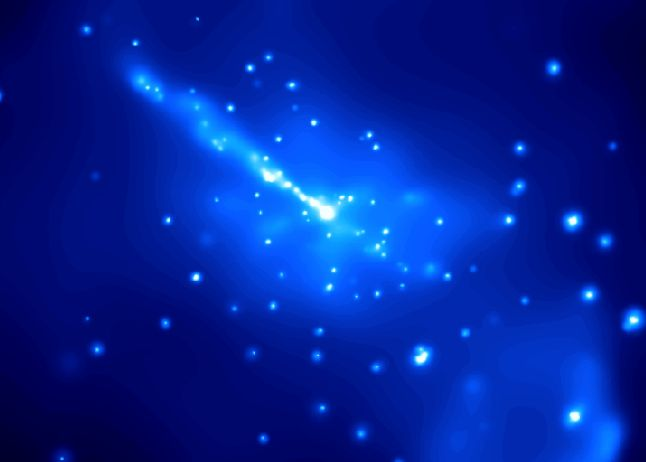
\includegraphics[width=1.1\linewidth]{images/cena_jet.jpg}
			Nearby galaxy Centaurus A in X-ray (Kraft et al 2001, Goodger et al 2010)
				\begin{block}{Entrainment in FRIs}
				Protons or heavier elements (stellar winds, clouds, SN, ambient medium) \\
			    $\rightarrow$ inexorable mass-loading and deceleration
						of the jet (De Young 1986, Bowman et al. 1996)
			\end{block}

		\end{column}
		\begin{column}{0.5\textwidth}
			\centering
			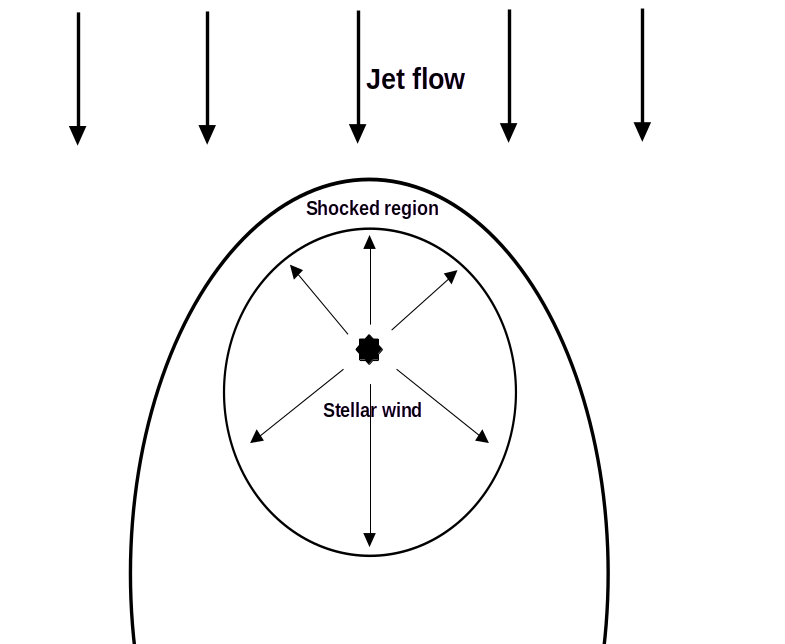
\includegraphics[width=.9\linewidth]{images/jet_wind.png}
				\begin{exampleblock}{Shocks}
				\begin{itemize}
					\item Balance between 2 supersonic matching flows (Komissarov 1994, Hubbard \& Blackman 2006)
					\item Conversion of $E_{k}$ into $U$ \\
						$\rightarrow$ expansion of the shock surface  \\
					\item Acceleration of $e^{-}$, $p$ or heavier ions\\
						$\rightarrow$ possible emissions up to $\gamma$-rays and
						acceleration of UHECR?
				\end{itemize}
			\end{exampleblock}

		\end{column}
	\end{columns}
	}
\end{frame}

\begin{frame}{Jet/star interaction time scale with the distance from the jet base}
	\begin{columns}
		{\scriptsize
		\begin{column}{0.5\textwidth}
			\begin{alertblock}{Close to the AGN | $z<10\,{\rm pc}$}
				\begin{itemize}
					\item Presence of large amounts of gas \\
						$\rightarrow$ lots of stars (RG, MS, AGB..) 
					\item Interaction with the outflow short ($t_{\rm int}=2R_{\rm j}/v_{\rm orb}$, typically 
							$\approx {\rm kyr}$)
								but frequent (short orbital period) (Kurfürst et al. 2024)\\
						$\rightarrow$ small mass loss per interaction  \\
				\end{itemize}
			\end{alertblock}
			\begin{block}{Far from the AGN | $z>{\rm kpc}$}
				\begin{itemize}
					\item The jet has expanded \\
							$\rightarrow$ Jet/star interaction time scale increases
								(typ. $\approx{\rm Myr}$)
					\item Stellar population typ. $\approx 1 {\rm star/pc}^{3}$ \\
						$\Rightarrow$ If SRG, eventual explosion
				\item 70 SN/century and ~0.01\% of them inside the jet (Vieyro et al. 2019)
				\end{itemize}
			\end{block}
		\end{column}
		\begin{column}{0.5\textwidth}
			\centering
			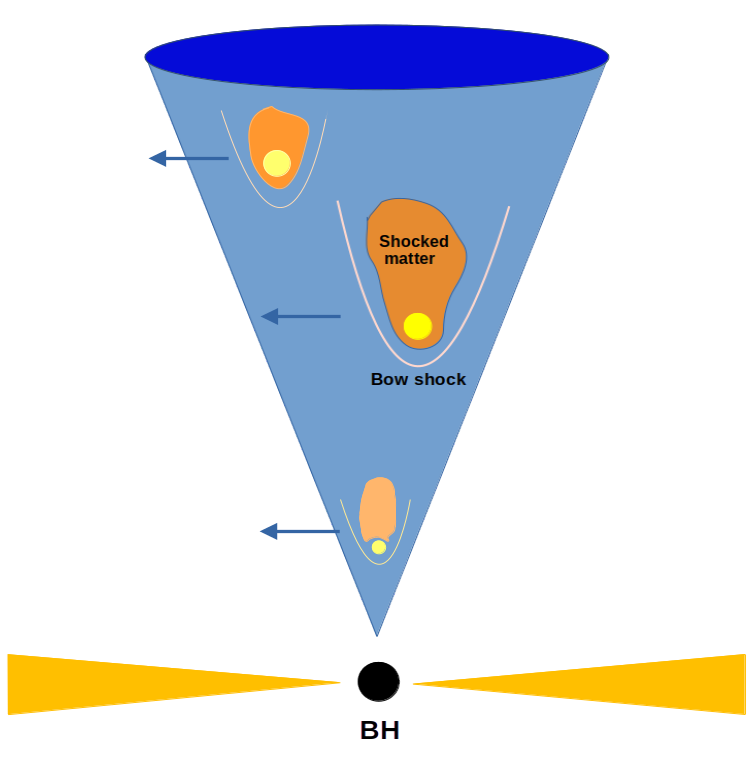
\includegraphics[width=\linewidth]{images/jet_mobstacles.png}
			\bf{A SRG can explode within the jet flow (Bosch-Ramon 2023) \\
		If the jet ram pressure becomes dominant over the SN remnant \\
						$\Rightarrow$ eventual disruption	}

		\end{column}}	
	\end{columns}
\end{frame}
